\documentclass[12pt]{article}                         
\pagestyle{plain} %-- Document Set Up Command

%-- Document Setup & Layout
\usepackage{fancyhdr}
\usepackage{comment}
\usepackage{multicol}
\usepackage[
  letterpaper,
  left=1in,
  right=1in,
  textheight=9.5in,
  bmargin=0.75in  % Adjust this value to push the footer down
]{geometry}

%-- Color & Text Formatting
\usepackage[svgnames]{xcolor} 
\usepackage{textcomp}
\usepackage{ulem}

%-- Math Packages
\usepackage{amsmath}     
\usepackage{amsfonts}
\usepackage{amstext}
\usepackage{amssymb}
\usepackage{latexsym}
\usepackage{bm}

%-- Graphics and Figures
\usepackage{graphicx}    
\usepackage{tikz}
\usepackage{pgfplots}
\usepackage{circledtext}
\usepackage{float}
\usetikzlibrary{arrows.meta}
%-- Tables
\usepackage{array}      
\usepackage{tabularx}

%-- Lists
\usepackage{enumitem}    
%\usepackage{enumerate}
\usepackage{tasks}

%-- TikZ Libraries
\usetikzlibrary{shapes.geometric} 

%-- Header/Footer
\pagestyle{fancy}
\fancyhf{} % Clear all header and footer fields
\fancyhead[L]{Jack Lingbeck} % Left header with name
\fancyhead[R]{Janurary 30th, 2026} % Right header with date
\renewcommand{\headrulewidth}{0.4pt} % Horizontal line below the header
\rfoot{Page \thepage}
\lfoot{Homework 1 Unit 1}

\begin{document}
\large
\begin{center}
\fbox{\begin{tabular}{c}
\bf Math 675 Spring 2026: \\
\bf Homework 1 Unit ? \\
\bf Due Tuesday, Janurary 3rd, 2026\\
\end{tabular}}
\end{center}

\section*{Question 1:}
For each system of differential equations in a-d below
\begin{itemize}
\item Plot the change vector using the points $(1,1),(1,-1),(-1,-1),(-1,1)$
\item Use the vector field to classify the equilibrium point(s) as stable, \\ unstable, a saddle point, an unstable spiral,
a stable spiral, or a center.
\end{itemize}
%\begin{minipage}[t]{0.45\textwidth}
\begin{enumerate}
    \item[(a)] $x' = -x, \quad y' = -5y$ \\
    Coupled: No;   \\ 
    EPs: Set $x'=0, y'=0$ \\
    $\left\{\begin{alignedat}{3} -x & &&= 0 \\ & -5y &&= 0\end{alignedat}\right.
	\rightarrow
    \left\{\begin{alignedat}{3} x && = 0 \\ y &&= 0\end{alignedat}\right.
	$ \\
    Thus, the EP is $(0,0)$
    \\
    \begin{center}
    \renewcommand{\arraystretch}{1.2} % Adds a little vertical breathing room
    \begin{tabular}{ |c|c| } 
    \hline
    $(x,y)$ & $(x',y')=(-x,-5y)$ \\
    \hline 
    $(1,1)$   & $(-(1),-5(1))=(-1,-5)$ \\ 
    $(1,-1)$  & $(-(1),-5(-1))=(-1,5)$ \\ 
    $(-1,-1)$ & $(-(-1),-5(-1))=(1,5)$   \\ 
    $(-1,1)$  & $(-(-1),-5(1))=(1,-5)$  \\ 
    \hline
    \end{tabular}
    \end{center}

    \item[(b)] $x' = 4x - y, \quad y' = 2x + y$ \\
    Coupled: Yes;  \\ 
    EPs: Set $x'=0, y'=0$ \\
    $\left\{\begin{alignedat}{3} 4x &{}-{} y &&{}={} 0 \\ 2x &{}+{} y &&{}={} 0\end{alignedat}\right.
	\rightarrow
    \left\{\begin{alignedat}{3} 4x &  && = y \\ 2x &+ y &&= 0\end{alignedat}\right.
	\rightarrow \\
    \left\{\begin{alignedat}{3} 4x &  && = y \\ 2x &+ 4x &&= 0\end{alignedat}\right.
	\rightarrow
    \left\{\begin{alignedat}{3} 4x &  && = y \\ 6x &  &&= 0\end{alignedat}\right.
	\rightarrow
    \left\{\begin{alignedat}{3} y && = 0 \\ x &&= 0\end{alignedat}\right.
	$ \\
    Thus, the EP is $(0,0)$
    \\
%\end{enumerate}
%\end{minipage}
%\hfill
%\begin{minipage}[t]{0.45\textwidth}
%\begin{enumerate}
    \item[(c)] $x'_1 = x_2, \quad x'_2 = -2x_1 - 3x_2$ \\
    Coupled: Yes; \\    
    $\left\{\begin{alignedat}{3} &{}-{} \hphantom{1}x_2 &&{}={} 0 \\ -2x_1 &{}-{} 3x_2 &&{}={} 0\end{alignedat}\right.
	\rightarrow
    \left\{\begin{alignedat}{3} &{}\hphantom{-3}{} \hphantom{3} x_2 &&{}={} 0 \\ -2x_1 &{}-{} 3x_2 &&{}={} 0\end{alignedat}\right.
	\rightarrow \\
    \left\{\begin{alignedat}{3} &{}\hphantom{-3}{} \hphantom{3} x_2 &&{}={} 0 \\ -2x_1 &{}{} &&{}={} 0\end{alignedat}\right.
	\rightarrow
    \left\{\begin{alignedat}{3} x_1 && = 0 \\ x_2 &&= 0\end{alignedat}\right.
	$ \\
    Thus, the EP is $(0,0)$
    \\
    \item[(d)] $x' = 5x + 2y, \quad y' = -17x -5y$ \\
    Coupled: Yes;  \\ 
    EPs: Set $x'=0, y'=0$ \\
    $\left\{\begin{alignedat}{3} 4x &{}-{} y &&{}={} 0 \\ 2x &{}+{} y &&{}={} 0\end{alignedat}\right.
	\rightarrow
    \left\{\begin{alignedat}{3} 4x &  && = y \\ 2x &+ y &&= 0\end{alignedat}\right.
	\rightarrow \\
    \left\{\begin{alignedat}{3} 4x &  && = y \\ 2x &+ 4x &&= 0\end{alignedat}\right.
	\rightarrow
    \left\{\begin{alignedat}{3} 4x &  && = y \\ 6x &  &&= 0\end{alignedat}\right.
	\rightarrow
    \left\{\begin{alignedat}{3} y && = 0 \\ x &&= 0\end{alignedat}\right.
	$ \\
    Thus, the EP is $(0,0)$
    \\
\end{enumerate}
%\end{minipage}

\section*{Question 2:}
Let $a \in \mathbb{R}$ be a parameter. Consider the system of differential equations
$$x'(t) = 2x, \quad \quad y'(t) = ay$$
\begin{itemize}
\item[(a)] Use separation of variables to find the explicit solution for this system.
\item[(b)] Sketch the phase portrait for this system for the following values of \\ a: -1, 0, 1, 2. Do not use technology
for this part.
\item[(c)] Now use tech (Mathematica, Python, etc) to plot a complete vector field and some trajectories.
\item[(d)] Use the vector field to classify the equilibrium point(s) as stable, unstable, a saddle point, an unstable spiral,
a stable spiral, or a center.
\end{itemize}
\centering % Center the TikZ picture within its minipage
    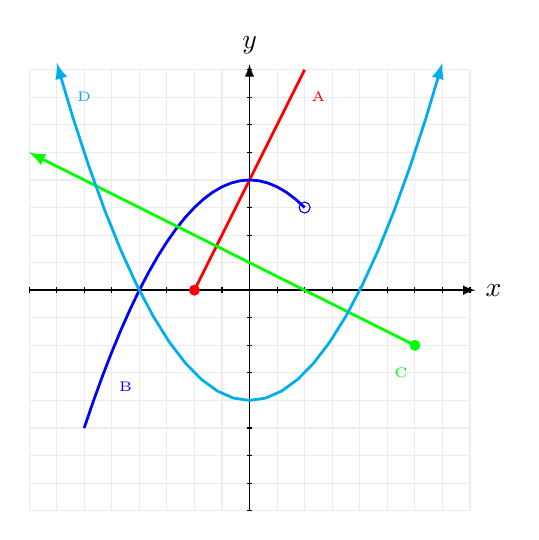
\begin{tikzpicture}[scale=0.35]
        \draw[gray!15,step=1cm] (-8,-8) grid (8,8);
        \draw[line width=0.2mm, -latex] (-8,0) -- (8.2,0) node[right] {$x$};
        \foreach \x in {-8,...,8} \draw (\x,.1)--(\x,-.1);
        \draw[line width=0.2mm,  -latex] (0,-8) -- (0,8.2) node[above] {$y$};
        \foreach \y in {-8,...,8} \draw (.1,\y)--(-.1,\y);
        
        \draw[red,line width=1pt] plot[domain= -2:2] (\x,{2*\x+4}) node[font=\tiny] at (2.5, 7) {A};
        \fill[red] (-2, 0) circle (0.2);
        \draw[blue,line width=1pt] plot[domain= -6:2] (\x,{-0.25*\x*\x+4}) node[font=\tiny] at (-4.5, -3.5) {B};
        \draw[blue] (2, 3) circle (0.2);
        \draw[green,line width=1pt, latex-] plot[domain= -8:6] (\x,{-0.5*\x+1}) node[font=\tiny] at (5.5, -3) {C};
        \fill[green] (6, -2) circle (0.2);
        \draw[cyan,line width=1pt, latex-latex] plot[domain= -7:7] (\x,{0.25*\x*\x-4}) node[font=\tiny] at (-6, 7) {D};    \end{tikzpicture}

\section*{Question 3:}
Let $a : R → R$ be a continuous function. Consider the first order ODE
$$x' = a(t)x$$
\begin{itemize}
\item[(a)] Find a formula involving integrals for the solution of this system. \\
$$ \frac{dx}{dt} = a(t)x(t)
\longrightarrow \int \frac{1}{x(t)} dx = \int a(t) dt$$
$$ \ln|x| $$
$$\int x dx$$
\item[(b)] Prove that your formula gives the general solution of this system. Hint: follow the sketch of proof done on
the first day of class
\end{itemize}
\end{document}